\documentclass[class=article,border=5pt,tikz]{standalone}
\usetikzlibrary{calc,intersections,backgrounds}

\begin{document}

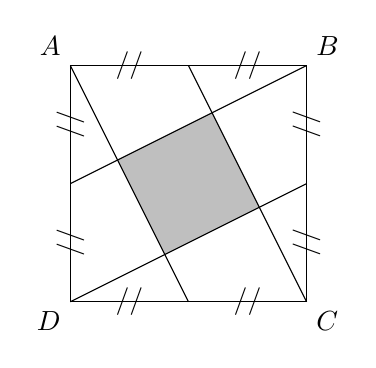
\begin{tikzpicture}[scale=3]
\coordinate (A) at (0,1);
\coordinate (B) at (1,1);
\coordinate (C) at (1,0);
\coordinate (D) at (0,0);
\coordinate (E) at (0.5,1);
\coordinate (F) at (1,0.5);
\coordinate (G) at (0.5,0);
\coordinate (H) at (0,0.5);
% Find intersection of EC and BH
\path[name path global=EC] (E) -- (C);
\path[name path global=BH] (B) -- (H);
\path [name intersections={of=EC and BH, by=I}];
% Find intersection of FD and CE
\path[name path global=FD] (F) -- (D);
\path[name path global=CE] (C) -- (E);
\path [name intersections={of=FD and CE, by=J}];
% Find intersection of GA and DF
\path[name path global=GA] (G) -- (A);
\path[name path global=DF] (D) -- (F);
\path [name intersections={of=GA and DF, by=K}];
% Find intersection of HB and AG
\path[name path global=HB] (H) -- (B);
\path[name path global=AG] (A) -- (G);
\path [name intersections={of=HB and AG, by=L}];

% Draw the main square and labels
\draw (A) node [above left] {$A$} -- 
      (E) node [midway] {//}--
      (B) node [midway] {//} node [above right] {$B$} -- 
      (F) node [midway,sloped] {//}--
      (C) node [midway,sloped] {//} node [below right] {$C$} -- 
      (G) node [midway] {//} --
      (D) node [midway] {//} node [below left] {$D$} -- 
      (H) node [midway,sloped] {//} --
          node [midway,sloped] {//} cycle;
      
% Draw the lines connecting the vertex to the opposite midpoint
\draw (E) -- (C);
\draw (F) -- (D);
\draw (G) -- (A);
\draw (H) -- (B);

\begin{pgfonlayer}{background}% background otherwise it 'leaks'
  \fill [color=gray, opacity=0.5] 
    (I) -- (J) -- (K) -- (L);
\end{pgfonlayer}

\end{tikzpicture}


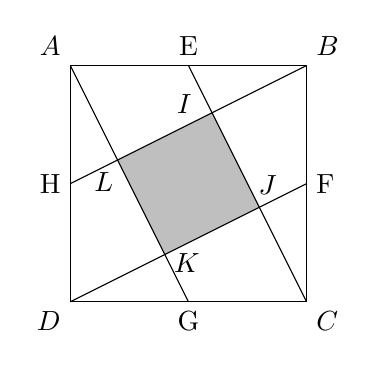
\begin{tikzpicture}[scale=3]
\coordinate (A) at (0,1);
\coordinate (B) at (1,1);
\coordinate (C) at (1,0);
\coordinate (D) at (0,0);
\coordinate (E) at (0.5,1);
\coordinate (F) at (1,0.5);
\coordinate (G) at (0.5,0);
\coordinate (H) at (0,0.5);
% Find intersection of EC and BH
\path[name path global=EC] (E) -- (C);
\path[name path global=BH] (B) -- (H);
\path [name intersections={of=EC and BH, by=I}];
% Find intersection of FD and CE
\path[name path global=FD] (F) -- (D);
\path[name path global=CE] (C) -- (E);
\path [name intersections={of=FD and CE, by=J}];
% Find intersection of GA and DF
\path[name path global=GA] (G) -- (A);
\path[name path global=DF] (D) -- (F);
\path [name intersections={of=GA and DF, by=K}];
% Find intersection of HB and AG
\path[name path global=HB] (H) -- (B);
\path[name path global=AG] (A) -- (G);
\path [name intersections={of=HB and AG, by=L}];

% Draw the main square and labels
\draw (A) node [above left] {$A$} -- 
      (E) node [above] {E} --
      (B) node [above right] {$B$} -- 
      (F) node [right] {F} --
      (C) node [below right] {$C$} -- 
      (G) node [below] {G} --
      (D) node [below left] {$D$} -- 
      (H) node [left] {H} --
          cycle;

% Draw the lines connecting the vertex to the opposite midpoint
\draw (E) -- (C);
\draw (F) -- (D);
\draw (G) -- (A);
\draw (H) -- (B);

% Label the vertices of the inscribed square
\node at (I) [shift={(-10pt,+3pt)}] {$I$};
\node at (J) [shift={(+3pt,+8pt)}] {$J$};
\node at (K) [shift={(+8pt,-3pt)}] {$K$};
\node at (L) [shift={(-5pt,-8pt)}] {$L$};

\begin{pgfonlayer}{background}% background otherwise it 'leaks'
  \fill [color=gray, opacity=0.5] 
    (I) -- (J) -- (K) -- (L);
\end{pgfonlayer}

\end{tikzpicture}


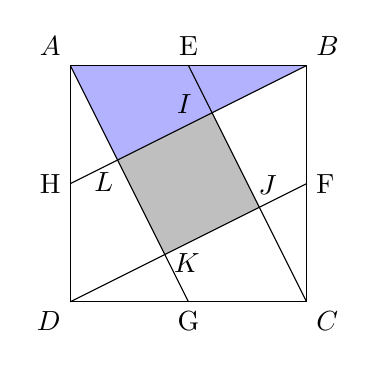
\begin{tikzpicture}[scale=3]
\coordinate (A) at (0,1);
\coordinate (B) at (1,1);
\coordinate (C) at (1,0);
\coordinate (D) at (0,0);
\coordinate (E) at (0.5,1);
\coordinate (F) at (1,0.5);
\coordinate (G) at (0.5,0);
\coordinate (H) at (0,0.5);
% Find intersection of EC and BH
\path[name path global=EC] (E) -- (C);
\path[name path global=BH] (B) -- (H);
\path [name intersections={of=EC and BH, by=I}];
% Find intersection of FD and CE
\path[name path global=FD] (F) -- (D);
\path[name path global=CE] (C) -- (E);
\path [name intersections={of=FD and CE, by=J}];
% Find intersection of GA and DF
\path[name path global=GA] (G) -- (A);
\path[name path global=DF] (D) -- (F);
\path [name intersections={of=GA and DF, by=K}];
% Find intersection of HB and AG
\path[name path global=HB] (H) -- (B);
\path[name path global=AG] (A) -- (G);
\path [name intersections={of=HB and AG, by=L}];

% Draw the main square and labels
\draw (A) node [above left] {$A$} -- 
      (E) node [above] {E} --
      (B) node [above right] {$B$} -- 
      (F) node [right] {F} --
      (C) node [below right] {$C$} -- 
      (G) node [below] {G} --
      (D) node [below left] {$D$} -- 
      (H) node [left] {H} --
          cycle;

% Draw the lines connecting the vertex to the opposite midpoint
\draw (E) -- (C);
\draw (F) -- (D);
\draw (G) -- (A);
\draw (H) -- (B);

% Label the vertices of the inscribed square
\node at (I) [shift={(-10pt,+3pt)}] {$I$};
\node at (J) [shift={(+3pt,+8pt)}] {$J$};
\node at (K) [shift={(+8pt,-3pt)}] {$K$};
\node at (L) [shift={(-5pt,-8pt)}] {$L$};

\begin{pgfonlayer}{background}% background otherwise it 'leaks'
  \fill [color=gray, opacity=0.5] 
    (I) -- (J) -- (K) -- (L);
\end{pgfonlayer}

\begin{pgfonlayer}{background}% background otherwise it 'leaks'
  \fill [color=blue, opacity=0.3] 
    (E) -- (I) -- (B);
\end{pgfonlayer}

\begin{pgfonlayer}{background}% background otherwise it 'leaks'
  \fill [color=blue, opacity=0.3] 
    (A) -- (E) -- (I) -- (L);
\end{pgfonlayer}


\end{tikzpicture}

\end{document}
